\documentclass[conference]{IEEEtran}
\usepackage[utf8]{inputenc}
\usepackage[spanish]{babel}
\usepackage{graphicx}
\usepackage{url}
\usepackage[hidelinks]{hyperref}
\usepackage{cite}

\title{Narrador de cuentos y novelas gráficas mediante aprendizaje automático}

\author{\IEEEauthorblockN{Maverick Chacón, Marny López, Kendall Méndez}
\IEEEauthorblockA{Universidad CENFOTEC\\
Email: {mchacon, mlopez, kmendez}@ucenfotec.ac.cr}}

\begin{document}

\maketitle

\begin{figure}[ht]
\centering
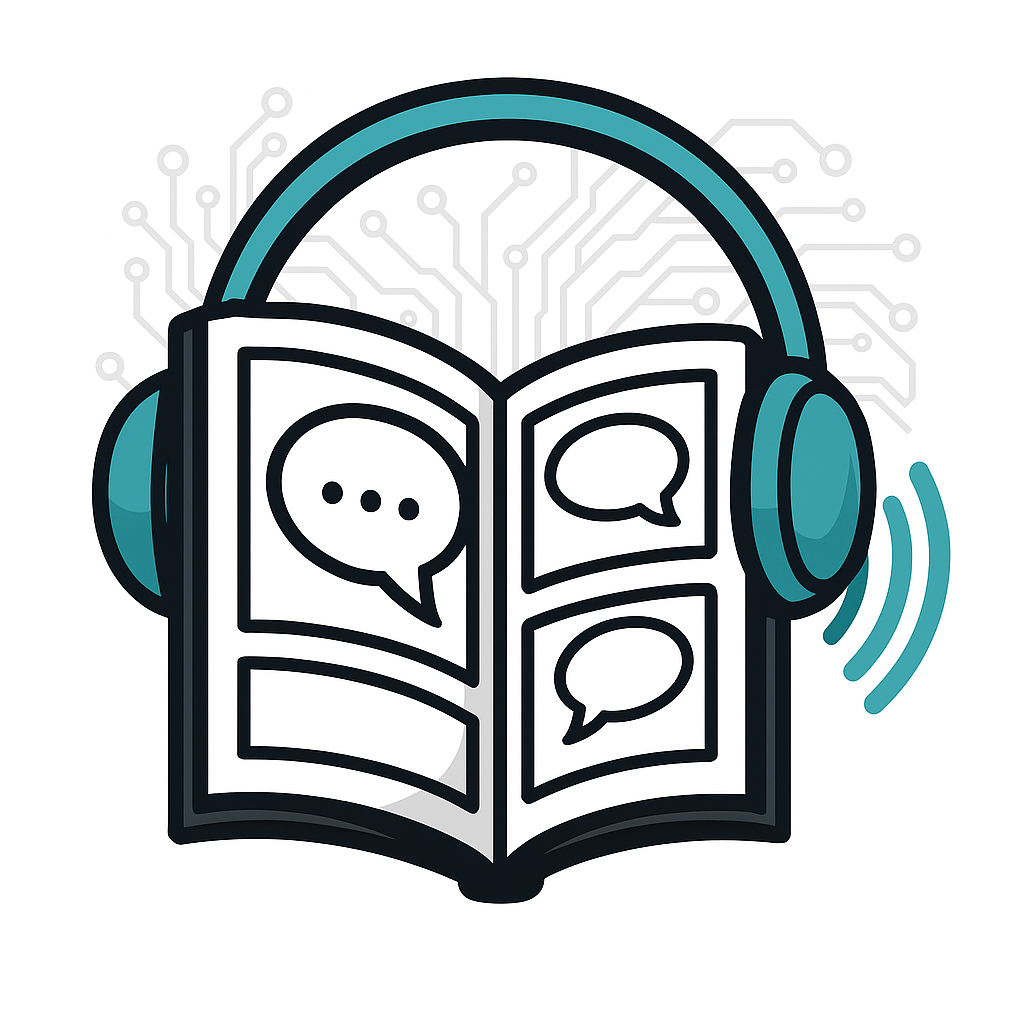
\includegraphics[width=0.3\columnwidth]{resources/mangAI.png}
\end{figure}

\begin{abstract}
Este trabajo presenta una herramienta basada en inteligencia artificial capaz de convertir contenido visual de mangas y novelas gráficas en narraciones orales accesibles para personas con discapacidad visual. El sistema combina detección de objetos (YOLOv8), reconocimiento óptico de caracteres (OCR), modelos de lenguaje (LLM) y conversión de texto a voz (TTS), implementado en una arquitectura modular y ejecutable localmente. El código fuente y la documentación completa están disponibles en: \url{https://github.com/iMrLopez/mangAI/}
\end{abstract}

\begin{IEEEkeywords}
Accesibilidad, OCR, YOLO, LLM, Text-to-Speech, Discapacidad Visual, Narración Automática
\end{IEEEkeywords}

\section{Introducción}
Las novelas gráficas y mangas son formas de arte narrativo que dependen fuertemente de lo visual. Esto presenta una barrera de accesibilidad significativa para personas ciegas o con baja visión. Nuestra propuesta busca abordar esta problemática mediante una herramienta capaz de interpretar y narrar automáticamente el contenido visual en formato de audio.

\section{Trabajos Relacionados}
Proyectos recientes han explorado la detección de paneles y burbujas de texto usando YOLOv8 \cite{yolov8comics}, mientras que OCR tradicional como Tesseract ha sido ampliamente utilizado en textos impresos \cite{smith2007tesseract}. Sistemas que combinan YOLO y OCR para accesibilidad visual han demostrado buenos resultados en la lectura de texto en imágenes \cite{patel2022ocrtts}.
En el ámbito de la accesibilidad digital, Sharma et al.\ \cite{sharma2021accesscomics} presentan AccessComics, un lector de cómics digitales accesible diseñado para personas con discapacidad visual. El sistema no emplea tecnologías OCR directamente, sino que se basa en cómics previamente segmentados mediante archivos SVG con metadatos estructurados. Utiliza síntesis de voz (Text-to-Speech) para narrar descripciones de escenas, diálogos y características de los personajes, asignando voces diferenciadas a cada uno. Aunque AccessComics no implementa reconocimiento óptico de caracteres en tiempo real, los autores reconocen el potencial de técnicas como OCR y visión por computadora para automatizar la preparación de cómics accesibles en versiones futuras. Este trabajo destaca la necesidad de herramientas basadas en IA que puedan procesar contenido visual complejo de forma autónoma y escalable.

\section{Metodología}
El sistema propuesto consta de los siguientes componentes:
\begin{itemize}
\item \textbf{YOLOv8}: para la detección de paneles y burbujas de diálogo en imágenes manga.
\item \textbf{OCR (PaddleOCR)}: para extraer texto de las regiones detectadas con filtrado por confianza.
\item \textbf{Modelos de Lenguaje (GPT-4 Vision y Text)}: para análisis visual de escenas y generación de narrativas estructuradas.
\item \textbf{TTS Multi-voz (ElevenLabs)}: para convertir el texto final en audio con voces diferenciadas para narrador y personajes.
\item \textbf{Streamlit}: para la interfaz web interactiva de carga de imágenes, configuración de parámetros y reproducción de audio.
\end{itemize}
El sistema implementa una arquitectura de procesamiento estructurada que organiza automáticamente las salidas en directorios con marca temporal, facilitando el seguimiento y gestión de resultados.

\begin{figure}[ht]
\centering
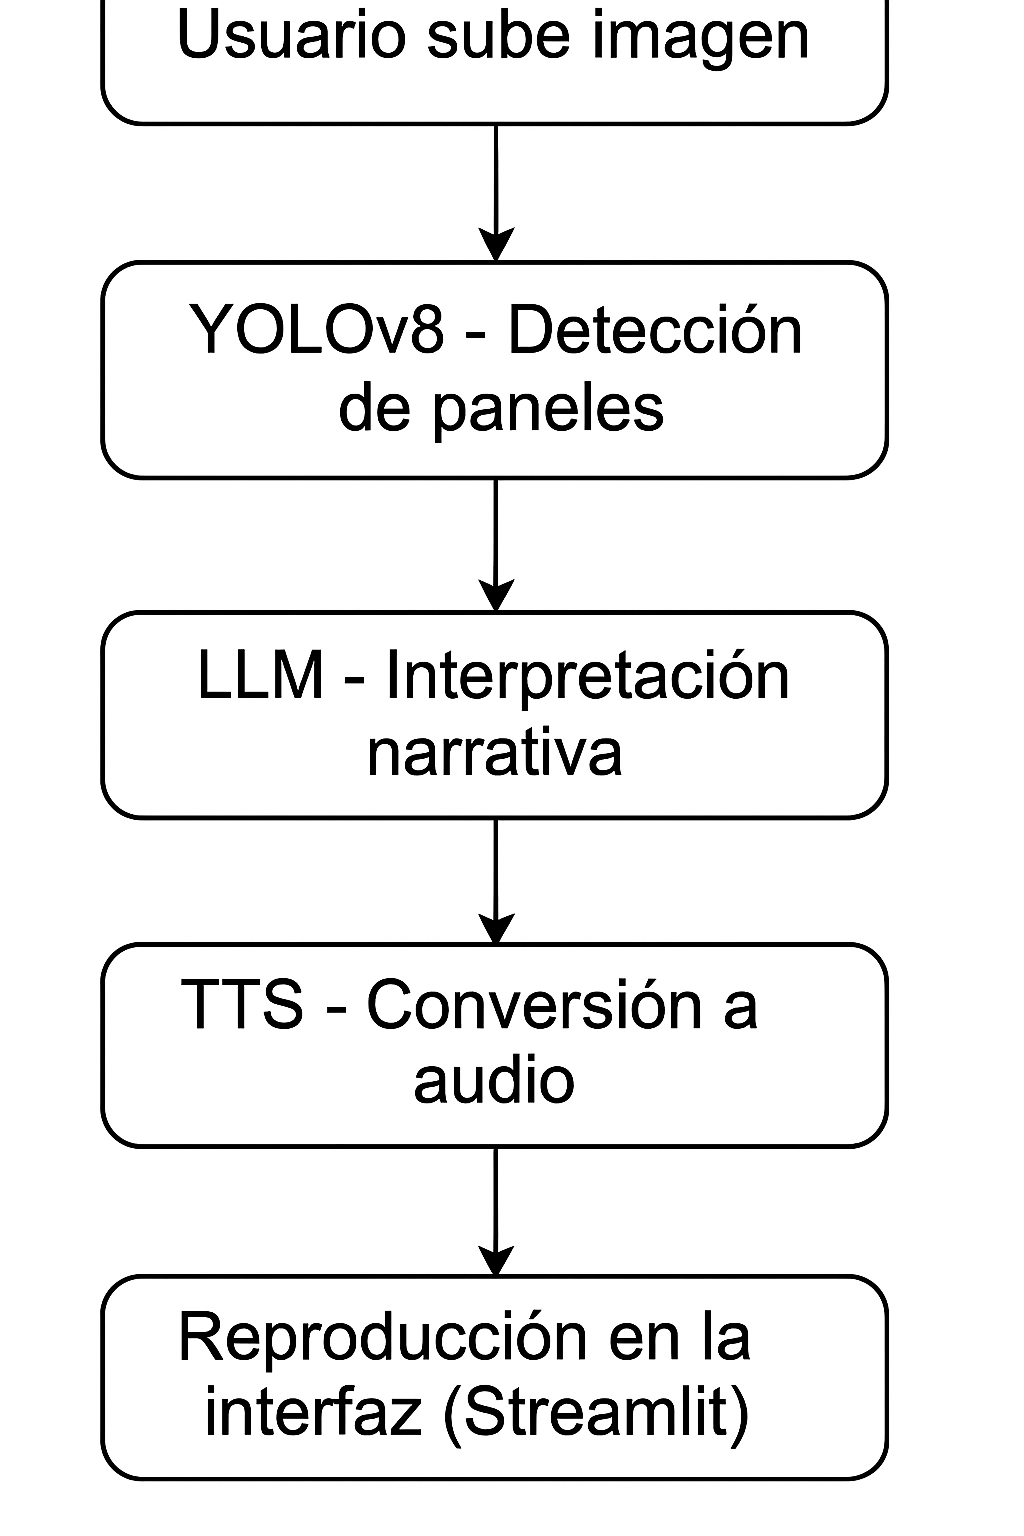
\includegraphics[width=0.25\textwidth]{resources/flujo_datos.png}
\caption{Flujo de procesamiento de datos en el sistema propuesto.}
\label{fig:flujo}
\end{figure}

\section{Resultados Esperados}
Se espera lograr una narración natural del contenido de mangas en formato de audio, manteniendo la coherencia narrativa y el orden correcto de los paneles (de derecha a izquierda, de arriba a abajo). Además, se anticipa que el uso de LLM permitirá enriquecer la narración con descripciones implícitas y emociones.

\section{Reconocimiento de texto}
\paragraph{El reconocimiento óptico de caracteres (OCR) es una tecnología clave para extraer texto de imágenes. En este artículo se compara el desempeño de dos herramientas ampliamente utilizadas: Tesseract OCR, desarrollado por Google, y PaddleOCR, parte del ecosistema de PaddlePaddle desarrollado por Baidu.}

\subsection{Comparación de Resultados entre Tesseract OCR y PaddleOCR en una Imagen de Prueba}

\paragraph{La comparación se realiza utilizando una imagen de una matrícula decorativa del estado de Florida [figura 1]. Visualmente, el texto "FLORIDA" incluye una ilustración de una naranja como parte de la letra "O". Esto representa un reto para los motores OCR debido a la interferencia visual.
}
\begin{figure}
    \centering
    
\includegraphics[width=0.5\linewidth]{resources/test.jpg}
    \caption{Imagen de prueba OCR}
    \label{fig:enter-label}
\end{figure}
\subsubsection{Resultados de Tesseract OCR}
\begin{verbatim}
    Welcome to
FL@RIDA
| THE SUNSHINE STATE
\end{verbatim}
\textbf{Análisis de resultados}
\begin{itemize}
    \item "FLORIDA" es interpretado como "FL@RIDA", un error común cuando se confunden letras con símbolos debido a diseños o elementos gráficos.
    \item Se detecta un símbolo "|" antes de la tercera línea.
    \item El resultado tiene buena detección de las tres líneas, pero con errores en caracteres específicos.
\end{itemize}

\subsubsection{Resultados de PaddleOCR}
\begin{verbatim}
Welcome to FLORIDA THE SUNSHINE STATE
\end{verbatim}
\textbf{Análisis de resultados}
\begin{itemize}
    \item El texto es correctamente reconocido, incluyendo "FLORIDA".
    \item No hay errores de sustitución de caracteres ni símbolos extraños.
    \item Toda la información es extraída en una sola línea, lo cual puede ser una ventaja o desventaja dependiendo del caso de uso.
\end{itemize}

\subsection{Mejoras en el preprocesamiento y postprocesamiento}
\paragraph{Para mejorar el rendimiento del sistema OCR, se aplicaron técnicas de preprocesamiento y postprocesamiento. Las imágenes de entrada fueron convertidas a escala de grises utilizando OpenCV, lo que permitió reducir el ruido y aumentar el contraste. Esta transformación fue seleccionada para simplificar la representación visual y facilitar la segmentación de caracteres por parte del motor OCR.
Tras la extracción del texto, se emplearon pasos de postprocesamiento con el fin de normalizar la salida. Se eliminó el espacio en blanco redundante y se corrigieron errores comunes de reconocimiento mediante sustituciones heurísticas. Por ejemplo, el carácter de barra vertical (|) fue reemplazado por la letra mayúscula I, y el dígito cero (0) por la letra O. Estas reglas permitieron mejorar la legibilidad del texto extraído sin requerir recursos lingüísticos adicionales.}

\subsection{Tecnología a utilizar}

\paragraph{Ambas herramientas ofrecen capacidades efectivas de reconocimiento de texto, pero PaddleOCR muestra mejor desempeño en este caso específico, al manejar correctamente elementos visuales decorativos y evitar errores de sustitución de caracteres. Sin embargo, la elección de la herramienta adecuada depende del contexto, el tipo de imágenes, y los requisitos del proyecto.}

\hypertarget{yolov8}{%
\section{YOLOv8}\label{yolov8}}

\subsection{Entrenamiento del modelo}\label{entrenamiento-del-modelo}
YOLOv8 permite entrenar modelos con datos de entrenamientos predefinidos. En este caso, se utilizó los datos de entrenamiento ``Manga109s'' \cite{aizawa2020manga109}, en donde se cuenta con alrededor de 109 volúmenes de manga. Esta base de datos incluye cuatro clases de objeto: persona, cara, texto y cuadro. Cada registro de clase incluye las coordenadas que indican la posición del objeto dentro de la página de manga. Las coordenadas siguen el formato: ``xmin, ymin, xmax, ymax''.

La arquitectura de YOLOv8 tiene las siguientes capas \cite{torres2025yolov8}:
\begin{itemize}
  \item \emph{Backbone Network:} Es la capa que extrae patrones como figuras, bordes, texturas, etc. Puede ser configurada para correr tareas más complejas o para priorizar velocidad sobre precisión según la aplicación.
  \item \emph{Neck Architecture:} Es la etapa encargada de ajustar la información extraída para poder detectar posteriormente objetos de diferentes tamaños.
  \item \emph{Detection Head:} Esta capa se encarga de clasificar objetos y tomar decisiones finales. Predice el centro del objeto con su respectiva altura y ancho.
\end{itemize}

Debido a que esta arquitectura predice el centro del objeto con su respectiva altura y ancho, el formato de los datos de entrenamiento tuvo que ser adaptado para poder utilizar los modelos de YOLOv8. El centro y las dimensiones de los objetos fueron calculados de la siguiente manera:

\[width = x_{\max} - x_{\min}\]
\[height = y_{\max} - y_{\min}\]
\[x_{center} = \frac{x_{\min} + \frac{width}{2}}{\mathrm{page}_{width}}\]
\[y_{center} = \frac{y_{\min} + \frac{height}{2}}{\mathrm{page}_{height}}\]

\subsection{Resultados obtenidos}\label{resultados-obtenidos}
% (contenido original sin cambios)
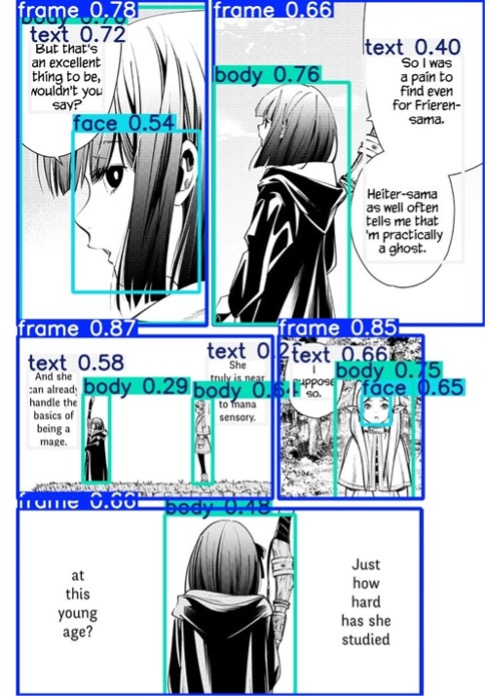
\includegraphics[width=2.20231in,height=3.158in]{resources/Picture1.jpg}

% ... (resto del contenido de resultados sin cambios)

\begin{table}[h!]
\centering
\small
\begin{tabular}{|c|c|c|c|c|}
\hline
\textbf{Run} & \textbf{Modelo} & \textbf{Epochs} & \textbf{Clases} & \textbf{Bloss} \\
\hline
1 & Yolov8s & 50 & 4 & 0.773 \\
2 & Yolov8l & 50 & 4 & 0.697 \\
3 & Yolov8l & 30 & 1 & 0.238 \\
\hline
\end{tabular}
\caption{Configuración y pérdida de caja (Bloss) para diferentes entrenamientos de YOLOv8}
\label{tab:yolov8-config}
\end{table}

\begin{table}[h!]
\centering
\small
\begin{tabular}{|c|c|c|c|}
\hline
\textbf{Run} & \textbf{Closs} & \textbf{DFL Loss} & \textbf{mAP50-95} \\
\hline
1 & 0.843 & 0.983 & 0.646 \\
2 & 0.671 & 0.981 & 0.737 \\
3 & 0.177 & 0.844 & 0.956 \\
\hline
\end{tabular}
\caption{Métricas de pérdida y precisión para los entrenamientos de YOLOv8}
\label{tab:yolov8-metrics}
\end{table}

\section{Secuencia de cuadros}
% (contenido original sin cambios)

\section{Construcción de la narrativa de la historia}
En las secciones anteriores se describió los procesos seguidos para identificar los cuadros de cada imagen, extraer el texto y ordenarlos. El siguiente paso corresponde a construir la narrativa de la historia previo a ser convertido a audio.

Para ello, se tomaron varias consideraciones. Según \cite{sharma2021accesscomics}, entre los aspectos más importantes al describir una historia se encuentran la descripción de la escena, la caracterización de personajes y el texto. Con base en esta información, se elaboró un \emph{prompt} para guiar a los modelos en la construcción de la narrativa de cada cuadro.

Además, se siguió una metodología inspirada en trabajos previos sobre cómics accesibles \cite{sharma2021accesscomics}, en donde en la narrativa se incluyeron roles asociados a los diálogos o descripciones de la escena con el fin de proporcionar mayor riqueza en el audio final.

El proceso de construcción de narrativa utiliza GPT-4 Vision para analizar el contenido visual de cada cuadro, identificando elementos como escenarios, personajes, emociones y acciones. Posteriormente, GPT-4 Text combina esta información visual con el texto extraído por OCR para generar una narrativa cohesiva que incluye tanto diálogos como descripciones contextuales, estructurada en roles de narrador y personajes.

\section{Generación de Audio Multi-voz}
La conversión de texto a voz representa el componente final del pipeline de procesamiento. El sistema implementa una solución de TTS multi-voz utilizando la API de ElevenLabs, que permite asignar voces diferenciadas a distintos roles narrativos.

\subsection{Arquitectura de TTS}
El módulo de TTS procesa la narrativa estructurada generada por los modelos de lenguaje, identificando automáticamente los segmentos correspondientes a narrador y personajes. Esta segmentación permite generar:
\begin{itemize}
\item \textbf{Audio del narrador}: Descripción de escenas, contexto y elementos visuales
\item \textbf{Audio de personajes}: Diálogos y expresiones de los personajes
\item \textbf{Audio combinado}: Mezcla sincronizada de ambas pistas para reproducción unificada
\end{itemize}

\subsection{Configuración de Voces}
La configuración del sistema permite especificar identificadores de voz específicos para cada rol:
\begin{itemize}
\item \texttt{ELEVENLABS\_NARRATOR\_VOICE\_ID}: Voz dedicada para descripciones narrativas
\item \texttt{ELEVENLABS\_CHARACTER\_VOICE\_ID}: Voz dedicada para diálogos de personajes
\end{itemize}

Esta separación de roles mejora significativamente la experiencia auditiva, proporcionando claridad en la distinción entre narración contextual y diálogos directos, elementos cruciales para la comprensión de contenido visual por parte de usuarios con discapacidad visual.

\section{Interfaz de Usuario con Streamlit}
La interfaz web desarrollada en Streamlit proporciona una experiencia de usuario intuitiva para la conversión de manga a audio. El sistema web integra todos los componentes de procesamiento en un flujo de trabajo cohesivo.

\begin{figure}[ht]
\centering
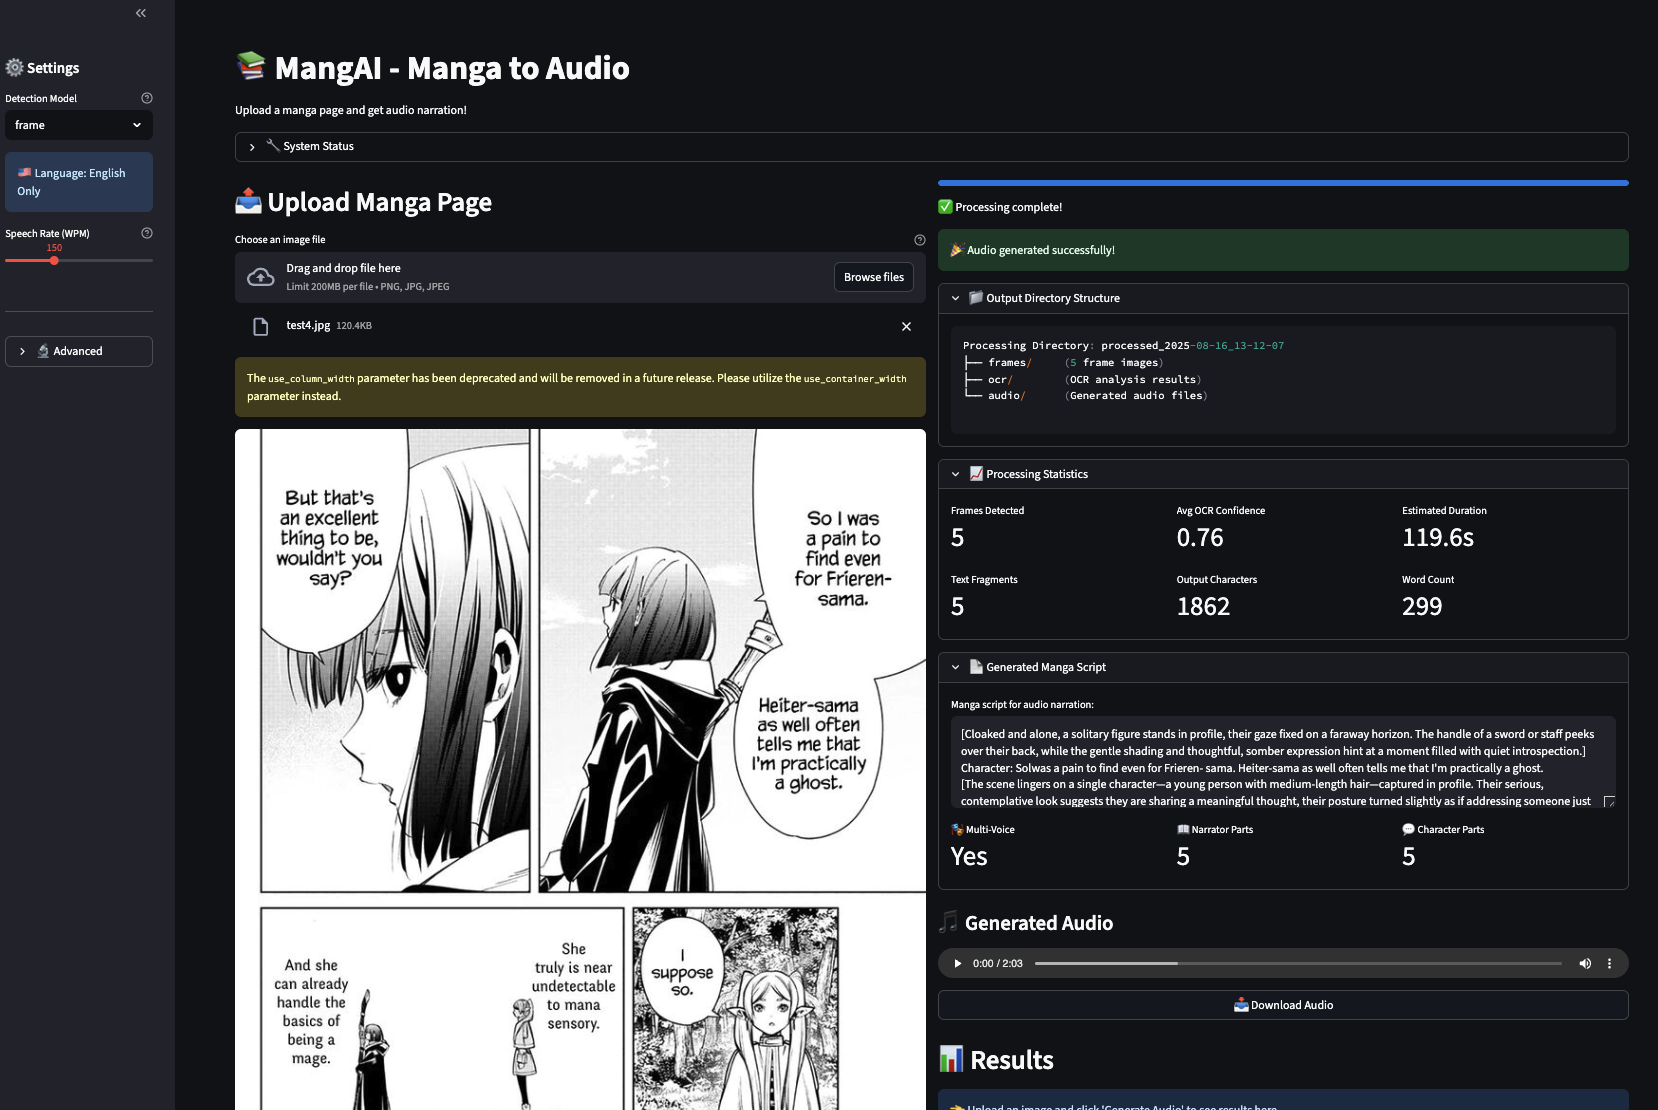
\includegraphics[width=\columnwidth]{resources/app.png}
\caption{Interfaz web de la aplicación MangAI desarrollada en Streamlit}
\label{fig:streamlit-interface}
\end{figure}

\subsection{Características de la Interfaz}
La aplicación web incluye las siguientes funcionalidades principales:
\begin{itemize}
\item \textbf{Carga de imágenes}: Soporte para formatos PNG, JPG y JPEG con validación automática
\item \textbf{Configuración de parámetros}: Selección de modelos YOLO y ajuste de umbrales de confianza
\item \textbf{Procesamiento en tiempo real}: Visualización del progreso de cada etapa del pipeline
\item \textbf{Resultados interactivos}: Reproducción de audio multi-voz con controles independientes
\item \textbf{Gestión de archivos}: Descarga de archivos de audio individuales y transcripciones completas
\end{itemize}

\subsection{Flujo de Trabajo de Usuario}
El flujo de trabajo implementado en la interfaz sigue una secuencia lógica:
\begin{enumerate}
\item \textbf{Selección de imagen}: El usuario carga una página de manga
\item \textbf{Configuración}: Ajuste de parámetros de procesamiento (modelo YOLO, umbrales)
\item \textbf{Procesamiento automático}: Ejecución secuencial de detección de cuadros, OCR, análisis LLM y generación de TTS
\item \textbf{Visualización de resultados}: Presentación de estadísticas de procesamiento y controles de audio
\item \textbf{Interacción con audio}: Reproducción independiente o combinada de pistas de narrador y personajes
\end{enumerate}

\subsection{Organización de Resultados}
La interfaz implementa un sistema de organización automática de resultados mediante directorios con marca temporal (\texttt{processed\_YYYYMMDD\_HHMMSS/}) que contienen:
\begin{itemize}
\item \texttt{frames/}: Cuadros extraídos y ordenados
\item \texttt{ocr/}: Resultados de reconocimiento de texto en formato JSON y texto plano
\item \texttt{audio/}: Archivos de audio multi-voz y transcripciones
\end{itemize}

Esta organización facilita el seguimiento de procesamiento y permite al usuario acceder a resultados intermedios para análisis o modificaciones posteriores.

\section{Conclusiones}
El trabajo presentado demuestra la viabilidad de un sistema automatizado para la conversión de contenido manga a narrativas de audio accesibles. La integración exitosa de múltiples tecnologías de inteligencia artificial (YOLO, PaddleOCR, GPT-4, ElevenLabs) en una arquitectura modular proporciona una solución escalable y efectiva para la accesibilidad digital.

\subsection{Logros Principales}
Los principales logros del sistema desarrollado incluyen:
\begin{itemize}
\item \textbf{Procesamiento automatizado completo}: Desde la detección de cuadros hasta la generación de audio multi-voz sin intervención manual
\item \textbf{Calidad de reconocimiento superior}: PaddleOCR demostró mayor precisión que Tesseract en el reconocimiento de texto decorativo y estilizado
\item \textbf{Narrativa enriquecida}: La integración de GPT-4 Vision y Text permite generar descripciones contextuales que van más allá del texto extraído por OCR
\item \textbf{Audio multi-voz diferenciado}: La implementación de ElevenLabs TTS con roles específicos mejora significativamente la experiencia auditiva
\item \textbf{Interfaz de usuario intuitiva}: Streamlit proporciona una experiencia web accesible con controles de audio especializados
\end{itemize}

\subsection{Impacto en Accesibilidad}
El sistema contribuye significativamente a la inclusión digital de personas con discapacidad visual al:
\begin{itemize}
\item Automatizar completamente el proceso de conversión, eliminando la dependencia de transcripciones manuales
\item Proporcionar narraciones enriquecidas que incluyen tanto diálogos como contexto visual
\item Ofrecer múltiples formatos de salida (audio separado, combinado, transcripciones) para diferentes preferencias de usuario
\item Implementar una arquitectura escalable que puede procesarse localmente sin dependencia de servicios externos críticos
\end{itemize}

\subsection{Trabajo Futuro}
Las direcciones futuras de desarrollo incluyen:
\begin{itemize}
\item \textbf{Soporte multiidioma}: Extensión del sistema para procesar manga en japonés y otros idiomas
\item \textbf{Reconocimiento de emociones}: Integración de análisis de expresiones faciales para enriquecer la caracterización de personajes
\item \textbf{Personalización de voces}: Implementación de clonación de voz para mantener consistencia de personajes a través de múltiples páginas
\item \textbf{Optimización de rendimiento}: Implementación de procesamiento paralelo para reducir tiempos de generación
\item \textbf{Integración con lectores digitales}: Desarrollo de plugins para plataformas de manga digital existentes
\end{itemize}

\subsection{Consideraciones Técnicas}
El diseño modular de la arquitectura permite adaptabilidad y mantenimiento eficientes. El uso de APIs comerciales (OpenAI, ElevenLabs) proporciona calidad superior, mientras que la inclusión de alternativas de código abierto garantiza sostenibilidad a largo plazo. La organización estructurada de resultados facilita la auditoría y mejora continua del sistema.

En conclusión, este trabajo establece una base sólida para sistemas de accesibilidad automatizada en contenido visual narrativo, demostrando que la combinación adecuada de tecnologías de IA puede generar soluciones prácticas y efectivas para la inclusión digital.

\bibliographystyle{IEEEtran}
\bibliography{references}

\end{document}
